\documentclass[12pt]{article}
\usepackage{fullpage}
\usepackage{lscape}
\usepackage[top=2cm, bottom=4.5cm, left=2.5cm, right=2.5cm]{geometry}
\usepackage{amsmath,amsthm,amsfonts,amssymb,amscd}
\usepackage{lastpage}
\usepackage{enumerate}
\usepackage{fancyhdr}
\usepackage{mathrsfs}
\usepackage{xcolor}
\usepackage{graphicx}
\usepackage{subcaption}
\usepackage{listings}
\usepackage{hyperref}
\usepackage{titlesec}

\setcounter{secnumdepth}{4}
\titleformat{\paragraph}
{\normalfont\normalsize\bfseries}{\theparagraph}{1em}{}
\titlespacing*{\paragraph}
{0pt}{3.25ex plus 1ex minus .2ex}{1.5ex plus .2ex}

\hypersetup{%
  colorlinks=true,
  linkcolor=blue,
  linkbordercolor={0 0 1}
}

\lstdefinestyle{C++}{
    language        = C++,
    frame           = lines, 
    basicstyle      = \footnotesize,
    keywordstyle    = \color{blue},
    stringstyle     = \color{olive},
    commentstyle    = \color{red}\ttfamily,
    breaklines      = true,
    tabsize         = 2
}

\setlength{\parindent}{0.0in}
\setlength{\parskip}{0.05in}

\newcommand\code{\url}
\newcommand\course{COMP0023}
\newcommand\hwnumber{}                   
\newcommand\NetIDa{17134402}            \newcommand\NetIDb{-}            
\pagestyle{fancyplain}
\headheight 35pt
\lhead{\NetIDa}
\lhead{\NetIDa\\\NetIDb}                 
\chead{\textbf{\Large Assessment \hwnumber}}
\rhead{\course \\ \today}
\lfoot{}
\cfoot{}
\rfoot{\small\thepage}
\headsep 1.5em

\graphicspath{{./images/}}

\begin{document}

\section{}

\subsection{Single Packet Perspective}

Each network layer will have its separate effort to detect and correct error regarding any bit errors or packet corruptions.

\subsubsection{Physical Layer L1}

Errors are detected on the link via Error Control Coding (ECC) and can potentially further corrected by Forward Error Correction (FEC) methods. 

Slower Ethernet specifications (Fast Ethernet and Gigabit Ethernet) have limited error detection methods. For example, 8b/10b encoding used in Gigabit Ethernet does allow detecting single-bit errors, but no correction.

Later developments include ECC methods and an FEC sublayer. 10GBASE-R PHYs(IEEE 802.3ap) uses the 64b/66b encoding, which provides at least a 4-bit hamming distance protection for all payload. It also specifies an optional RS-FEC(2112, 2080) sublayer using the Reed–Solomon error correction algorithm. Furthermore, higher symbol rate PHY links have much stronger FEC methods in place. 100G backplane PHY(IEEE 802.3ap) deems FEC mandatory in higher-bitrate or longer-distance connections.

A packet with fewer bit errors on a PHY with FEC can potentially be corrected. If no FEC or longer burst errors happened, the PHY might deem the received encoding invalid and discard the packet.

\subsubsection{Link Layer L2}

The link layer, notably the Ethernet II, employs an FCS appending to the end of the packet before the interframe gap. It is calculated using a CRC32 algorithm, transmitting in little-endian bit order. It is a powerful algorithm that detects:
\begin{itemize}
    \item All burst errors of length $<= 31$
    \item All odd number of bit errors
    \item With high probability, burst errors of length $>= 32$
\end{itemize}

Although there are several types of research regarding using CRC to do error correction, it is still rare, and we can assume that a faulty frame detected would be dropped.

\subsubsection{Network Layer L3 and Transport Layer L4}

In Internet Protocol version 4 (IPv4), its checksum is a 1's complement checksum operating upon the IP header only. Its primary purpose is to ensure correctness in a multi-hop environment. It aims to detect errors in intermediate machines, which could potentially alter the IP header during packet transmission.

The TCP checksum is also 1's complement. It is enforced upon the TCP header, the TCP payload, and an IP pseudo-header. The IP pseudo-header includes the src/dst IP, TCP protocol number $\mathtt{0x06}$, and the IP size field from the lower level. It is meant to be an End-to-End (E2E) verification of the packet's integrity.

UDP checksum is optional upon UDP/IPv4 stack. Like TCP checksum, it is also a 1's complement of the header, payload and an IP pseudo-header. Contrary to IPv4, IPv6 does not have a checksum field. On a good note, no recalculation of checksum is needed upon forwarding packets. The L2 CRC and  L4 checksum would sufficiently check the L3 header. Hence, UDP/IPv6 has a mandatory checksum field.

1's complement is less powerful as it only guarantees single-bit error detection. It's primarily designed to work in a CPU-efficient (in bytes) and space-efficient (16 bits) way.

If the checksum detects an error in either (TCP/UDP)/(IPv4/IPv6), the packet would be dropped. In the rare case where L1-L4 ECC did not found the error, the corrupted packet would be sent to the upper layer.

\subsubsection{Summary}

In conclusion, the corrupted packet can either
\begin{itemize}
  \item gets corrected/dropped on PHY
  \item gets dropped on L2, L3, L4 if the checksum fails
  \item evades all checksums and gets passed on to the application
\end{itemize}

\subsection{End-To-End Perspective}

In the following discussions, we will divide each section into whether the corrupted bit is detected or not in ECCs of L1-L4.

\subsubsection{DNS transactions}

Upon typing \url{www.ucl.ac.uk} into the browser, the laptop would first query DNS to obtain the IP address. We assume the domain operates with DNS instead of DNSSEC.

\begin{itemize}
    \item Laptop looks up the DNS in cache. Since it's a new laptop, nothing would be found.
    \item Laptop sends a DNS request to a DNS server, usually a local/public DNS resolver.
    \item If found, the DNS reply containing \url{www.ucl.ac.uk}'s IP address would be replied.
    \item If not found, the DNS resolver would start resolving \url{www.ucl.ac.uk} from the root servers, all the way down to the authoritative nameservers (i.e. \url{dns-ns1.ucl.ac.uk}).
    \item Similarly, a DNS reply of \url{www.ucl.ac.uk} would be sent to the laptop.
\end{itemize}

\paragraph{Packet Error Detected}

The packet would most likely be discarded by a switch, router or server upon corruption. Then, the laptop browser would timeout on the query and resend it after a while. 

\paragraph{Packet Error Not Detected}

This rare case would result in either an invalid DNS query or a DNS query targetting a different domain. The common case would be an invalid DNS query. The name server or resolver shall detect this and drop this invalid DNS query. The rarer case would be the request reaching an entirely different authoritative server and getting either a \url{NXDOMAIN} reply or a reply on a different domain (i.e. \url{www.ual.ac.uk}). The laptop would found the response unrelated to its question. Hence, re-querying the DNS.

\subsubsection{HTTP transactions}

\url{www.ucl.ac.uk} shall be HTTP webpages (not Gopher). Although UCL serves only HTTP/1.1, \url{www.ucl.ac.uk/} also includes content served by CDN through HTTP/3, optionally. It's notable that HTTP/3 is based on QUIC/UDP/IP stack, while HTTP/1.1 on a TCP/IP stack. Moreover, when serving HTTPS/1.1, there's a TLS layer in between HTTP and TCP. We limit the scope to HTTP/TCP/IP stack in this question.

\paragraph{Packet Error Detected}

The TCP establishment includes three handshakes. If the laptop's packet corrupted on the first SYN or the third ACK, the server would not respond until the RTX timer runs out on the laptop and resends.

If any laptop's packet is corrupted during the transmission process, the RTX timer will timeout as the ACK will not happen. The laptop would then attempt to retransmit until ACKed.

The TCP teardown is comprised of four handshakes. If the first FIN from the laptop gets corrupted, the server would not reply with an ACK. After the RTX timeout, the laptop would resend FIN.

Suppose the fourth ACK (corresponding to server FIN) corrupts; the laptop would have already entered a TIME\_WAIT state, expecting to close the connection after 2 MSLs. However, the server would eventually reach RTX timeout as its FIN not ACKed. The server would retransmit a FIN to the laptop, reaching the laptop during TIME\_WAIT. The laptop will then retransmit ACK to the server and successfully close the connection.

\paragraph{Packet Error Not Detected}

In the rare case where the packet error is not detected, the serving application might receive a corrupted request. Typically, the HTTP request would be an invalid one. In the extreme case where the corrupted HTTP request is valid and contains a different URL, the server might respond with a 404 or with a wrong page. The server behaviour would be unpredictable in this case.


\newpage
\section{}

\renewcommand{\thesubsection}{\thesection.\alph{subsection}}

\subsection{}

\begin{figure}[h!]
  \makebox[\textwidth][c]{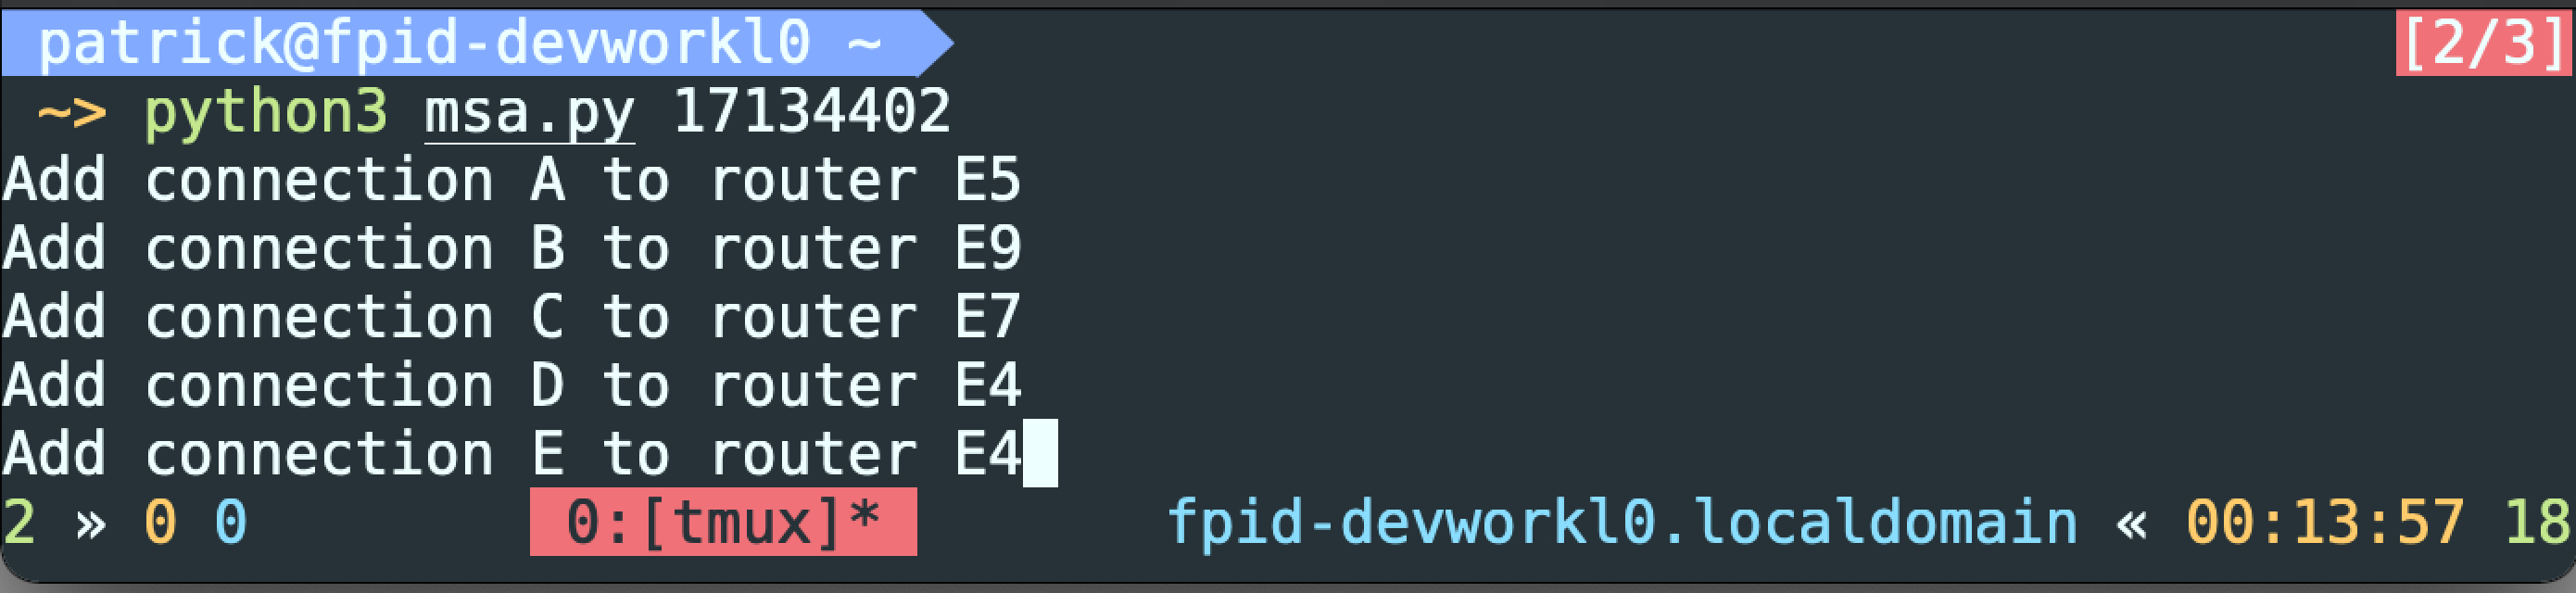
\includegraphics[width=\textwidth]{imgs/python-script-screenshot.png}}
  \caption{Python Script Screenshot}
  \label{fig:python-screenshot}
\end{figure}

\begin{figure}[h!]
  \makebox[\textwidth][c]{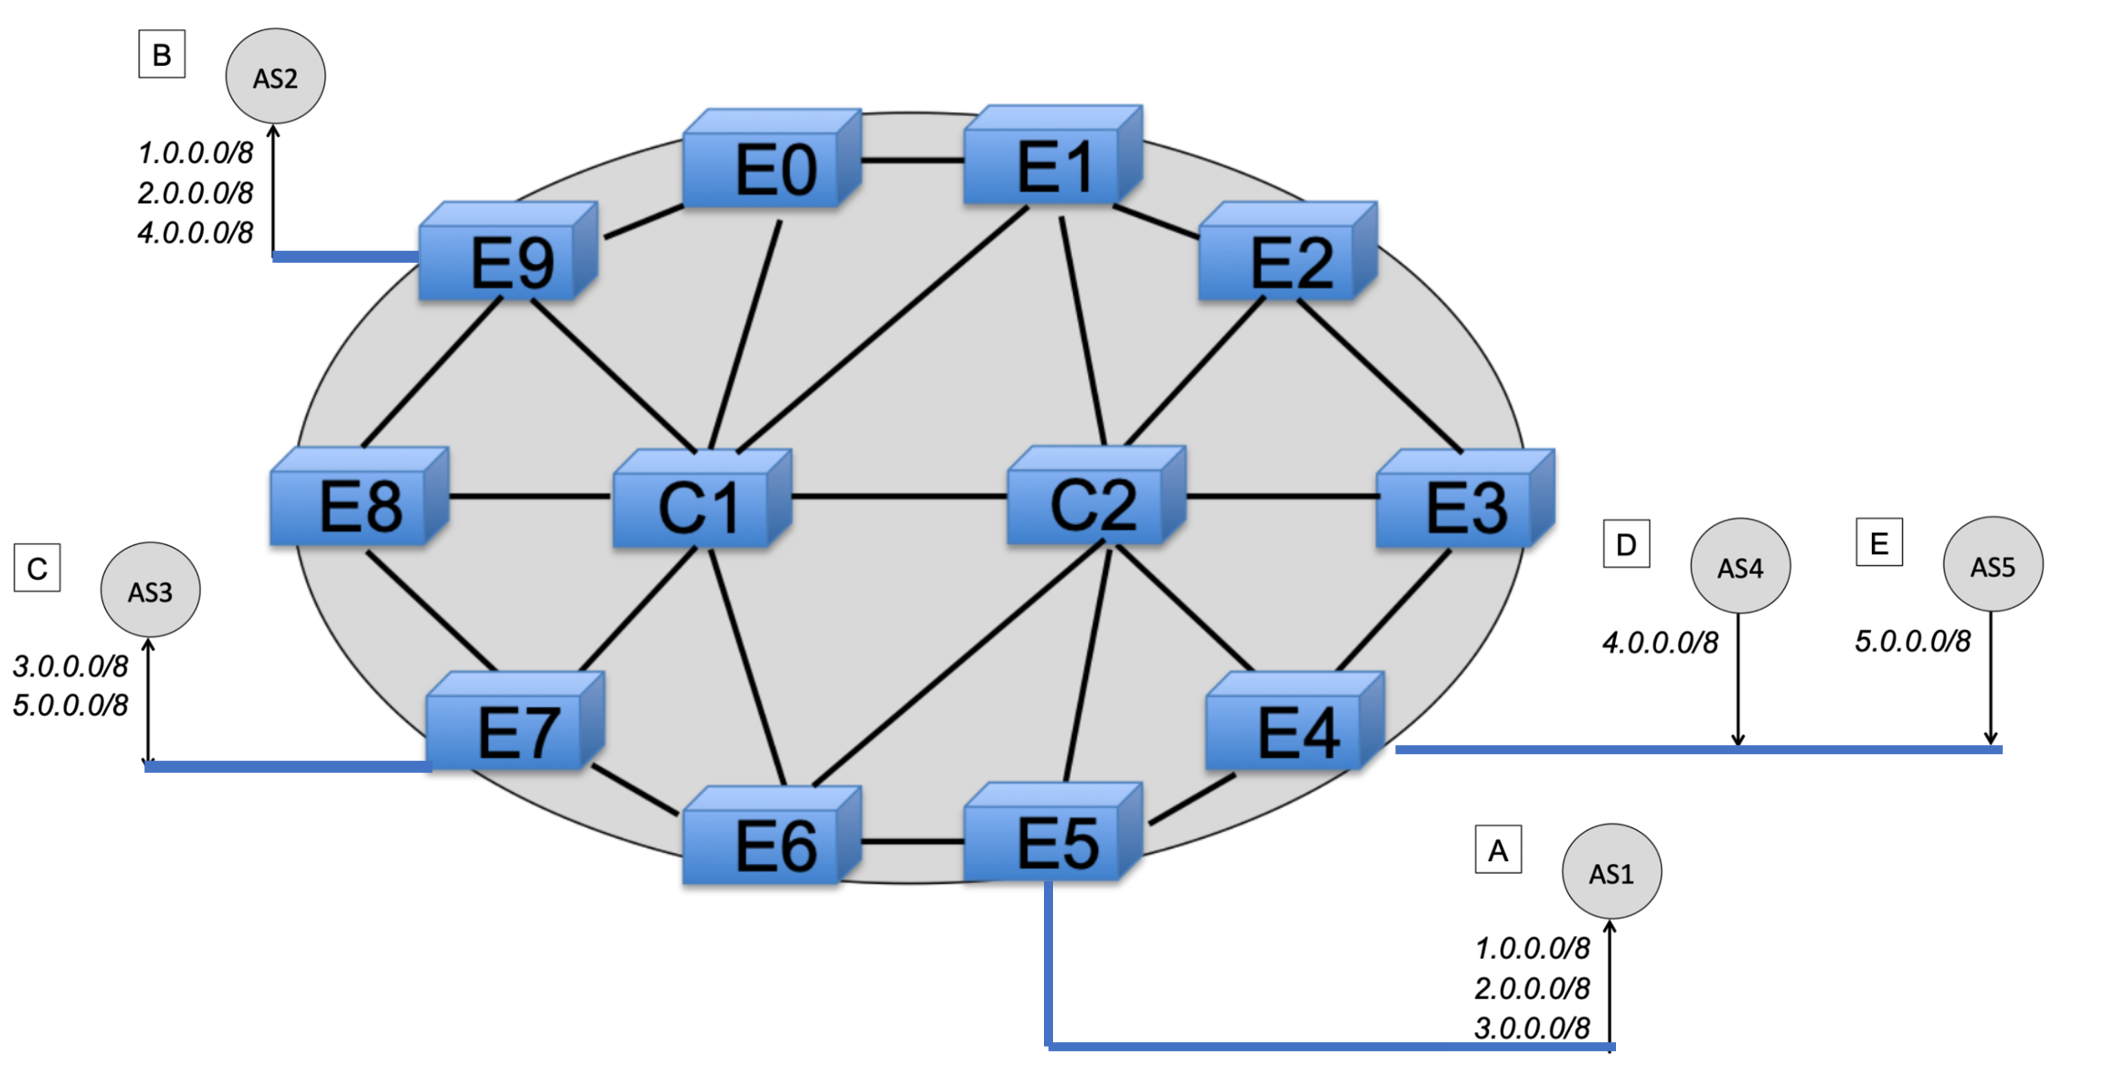
\includegraphics[width=1.1\textwidth]{imgs/topology.png}}
  \caption{Topology}
  \label{fig:topology}
\end{figure}

\subsection{}


C2 -> C1 -> E7
C1 -> C2 -> E4 5.0.0.0/8





AS-PATH length

if E9->C1->C2->E5, that implies AS1 has better AS-PATH length

then not possible to do E5->C2->C1->E9

vice versa, if E5->C2->C1->C9, AS1 must have 

i.e. 1.0.0.0/8








\end{document}